%
% chapter5.tex
%

\chapter{Experiments}\label{cha:experiments}
Paul Raatschen has performed a study\cite{raatschen:ipc} concluding that the original Fail2ban process can be improved upon.
It was determined that especially with many clients, Fail2ban struggled to keep up with high incoming traffic rates.
To remedy this issue, a more performant program, Simplefail2ban, was implemented and measured.
An increase in performance was evident.
Simplefail2ban supported two modes of \ac{IPC}.
The disk/file mode was akin to traditional file logging, while the shared memory approach would use a shared memory section to exchange data between processes.
A direct comparison between the already outlined socket approach and previously supported \ac{IPC} types necessitates the measurements in this chapter.

The following chapter details the measurements performed, outlining specifics according to Jain's
``The Art of Computer Systems Performance Analysis: Techniques For Experimental Design, Measurement, Simulation, and Modeling, NY\@: Wiley''\cite{jain:measurement} chapter 2.2.

\section{Test environment}
Two machines, both identical in hardware and software, were used in these experiments.
The first machine, the \ac{DUT}, ran Simplefail2ban and a test application responsible for receiving incoming traffic and reporting clients.
The second machine generated and sent traffic, consisting of both valid and invalid traffic, to the \ac{DUT} using TRex.

\begin{table}[b!]
    \renewcommand{\arraystretch}{1.5}
    \caption[Testbed specs]{Table of Hardware and Software parameters of the testbed.
    The first machine serves as the \ac{DUT}.
	The second machine generates traffic to be sent to the \ac{DUT} via TRex.}\label{tab:specs}
    \centering
    \small
    \begin{tabular}{ll}
        \toprule
        \multicolumn{2}{l}{\textbf{Hardware}} \\ \midrule
        CPU     & 16 $\times$ Intel(R) Xeon(R) Silver 4314 \ac{CPU} @ 2.40GHz \\
        NIC     & Mellanox Technologies MT2892 Family [ConnectX-6 Dx] \\
        RAM     & 128 GB \\ \bottomrule

        \multicolumn{2}{l}{\textbf{Software}} \\ \midrule
        OS          & Debian \ac{GNU}/Linux 11 \\
        Kernel      & 5.10.0-28-amd64 x86\_64 \\
        NIC Driver  & mlx5\_core; Version 5.8-2.0.3 \\
        TRex        & 2.99 (Stateless) \\ \bottomrule
    \end{tabular}
\end{table}

\section{Experimental design}
In his thesis\cite{raatschen:ipc}, Paul Raatschen showed that the shared memory mode of Simplefail2ban outperforms the traditional Fail2ban.
However, it remains unclear if the implementation of this \ac{IPC} type is more performant than other alternatives.
Specifically, the possibility of using Unix domain sockets as a mode of inter-process communication was not explored.
The following experiments enable a direct comparison between the two \ac{IPC} types.

\noindent
In general, the experiments consist of two participants and a one-sided data exchange.
The \ac{DUT}, or more specifically the application udp\_server, receives a stream of both wanted and unwanted data.
Identifying desired traffic is done by analyzing the message payload.
This is a crude and unrealistic approach to filtering malicious communication requests.
Such a simplification allows the application udp\_server to quickly generate log messages.
Since the goal of this study is to determine the most efficient \ac{IPC} type for Simplefail2ban, it is very plausible that this abstraction does not diminish the findings of this thesis.

\noindent
To compare the differing \ac{IPC} types, a set of performance metrics needs to be established:

\bigskip
\noindent
\textbf{Performance metrics}
\begin{itemize}
    \item Total number of unwanted requests dropped (number of packets)
    \item Total number of unwanted requests dropped, relative to the total amount of unwanted requests sent (percentage)
    \item Number of log messages processed by Simplefail2ban, relative to the number of log messages sent by the test server (percentage)
    \item \ac{CPU} utilization of Simplefail2ban (seconds of \ac{CPU} time)
\end{itemize}
Higher is better for the first three metrics.
The last metric should be minimized for the \ac{DUT} so its services are continually provided to valid clients.

\bigskip
\noindent
The fixed parameters for each of the experiments are the following\@:

\bigskip
\noindent
\textbf{Fixed parameters}
\begin{itemize}
    \item Hardware and Software parameters of the testbed in this table\@:
    \begin{itemize}
        \item \ac{CPU}\@: 16 cores, no hyper-threading enabled
        \item \ac{NIC}\@: Maximum transfer unit is 1500 bytes
        \item TRex\@: One interface, 30 threads
    \end{itemize}
    \item Number of entries in \ac{eBPF} maps for IPv4 \& IPv6\@: 1M
    \item Number of receiving threads used by udp\_server\@: 16
    \item Duration of measurement\@: 300 Seconds
    \item Amount of valid traffic sent\@: 50000 \ac{PPS}
    \item Number of clients sending valid traffic\@: 254
    \item \textbf{Simplefail2ban} parameters\@:
    \begin{itemize}
        \item Number of hash table bins used\@: 6000011
        \item Ban threshold for clients\@: 3
        \item Ban time for clients\@: 30 seconds
        \item Enabling the \ac{Regex} Matching feature of Simplefail2ban (the current implementation does not ban clients correctly when disabled)
        \item For \textbf{shared memory} specifically\@:
        \begin{itemize}
            \item Number of banning threads used\@: 16
            \item Line count for the shared memory buffer segments\@: 1M
            \item Segment count for the shared memory buffer\@: 16
            \item Overwrite feature enabled
            \item Workload stealing feature disabled
        \end{itemize}
        \item For \textbf{sockets} specifically\@:
        \begin{itemize}
            \item Number of banning threads used\@: 16
            \item Number of sockets\@: Same as number of reader processes (either one, or two when utilizing a second reader)
            \item Using default path to sockets created by the application\@: \texttt{tmp/}
            \item Using default socket receive and send buffer size configured on the system\@: 212992 Bytes
        \end{itemize}
        \item For \textbf{file} specifically\@:
        \begin{itemize}
            \item Number of banning threads used\@: 1 (file mode only supports one banning threads)
            \item Buffer size for uring\_getlines\@: 2048
        \end{itemize}
    \end{itemize}
\end{itemize}

\bigskip
\noindent
The factors, or variable parameters, during these experiments were the following\@:

\bigskip
\noindent
\textbf{Factors and their levels}
\begin{itemize}
    \item \ac{IP} stack: IPv4, IPv6 and IPv4/IPv6 mixed
    \item Effects of differing amount of invalid traffic sent: 100k, 1M, 10M, 20M, 30M \ac{PPS}
    \item Effects of differing number of clients sending invalid data: 65534 and 131068
    \begin{itemize}
        \item Range used for 65534 clients: 10.4.0.1 to 10.4.255.254 resulting in clients stemming from 256 subnets (using offset\_fixup of 5 for IPv6 in TRex script).
        \item Range used for 131068 clients: 10.4.0.1 to 10.5.255.252 resulting in clients stemming from 512 subnets (using offset\_fixup of 5 for IPv6 in TRex script).
        \item When using the IPv4/IPv6 \ac{IP} stack, the range for 65534 client is being used twice to generate both a IPv4 and IPv6 stream.
    \end{itemize}
    \item Differing \ac{IPC} type\@: FILE (traditional file-based logging), SHM (using shared memeory), SOCK (using unix domain sockets)
    \item For shared memory specifically:
    \begin{itemize}
        \item No 2nd Reader/ Enabling 2nd Reader
    \end{itemize}
    \item For sockets specifically:
    \begin{itemize}
        \item No 2nd Reader/ Enabling 2nd Reader
    \end{itemize}
\end{itemize}

\bigskip
\noindent
To generate the traffic being sent to the \ac{DUT}, TRex scripts are used.
These scripts provide the option to modify the sent traffic according to the factors outlined above.
During these measurements, adapted versions of Paul Raatschens\cite{raatschen:ipc} scripts were used.
To measure most performance metrics, an adaptation of the xdp\_ddos01\_blacklist\_cmdline program was used.
This application originally stems from Florian Mikolajczak master's thesis\cite{mikolajczak:ebpf} and routinely polls the number of dropped and passed packets from a specific \ac{eBPF} map.
It was modified by Paul Raatschen to output values as a \ac{csv} file.
The polled \ac{eBPF} map is ultimately used by Simplefail2ban to ban clients.
\ac{CPU} time was measured via the command top.

\section{Established Simplefail2ban \ac{IPC} types}
Software version changes warrant remeasurement of the shared memory and file \ac{IPC} mode for Simplefail2ban.
These will also be used to evaluate the newly implemented socket mode.

\subsection{Experiment 1a: Simplefail2ban Logfile}
It has already been shown that the file \ac{IPC} type of Simplefail2ban is outperformed by the shared memory mode.
Pure IPv4, IPv6 and a mixed IPv4/IPv6 \ac{IP} stack will be used.
File logging is expected to perform worse than the other \ac{IPC} types discussed in this thesis, and acts as a baseline for the other \ac{IPC} types.
In total, 25 unique measurements were conducted for this experiment.

\subsection{Experiment 1b: Simplefail2ban Shared Memory}
The newly implemented socket approach is intended to be a valid alternative to the shared memory mode of Simplefail2ban.
To enable a direct comparison, measurements for the shared memory mode need to be done under high enough loads, since with lower loads both the socket and shared memory mode are suspected to be performant enough.
All levels of invalid traffic rates are measured individually.
Again, either a pure IPv4, IPv6 or mixed IPv4/IPv6 \ac{IP} stack is utilized.
The most performant features will be used, meaning overwrite is enabled and workload stealing is disabled.
No second reader process is being employed here.
In total, 25 unique measurements were conducted for this experiment

\section{Measuring the socket \ac{API}}
In the following section, thorough variations of factors and their levels are used to evaluate the performance of the socket mode.
Also, heavy workloads are employed to determine how the socket mode performs in worst case scenarios.
This will allow for a direct comparison between socket and shared memory mode.
The data flow in the \ac{DUT} can be seen in \ref{fig:socket:measurement}.

\begin{figure}[h!]
    \centerline{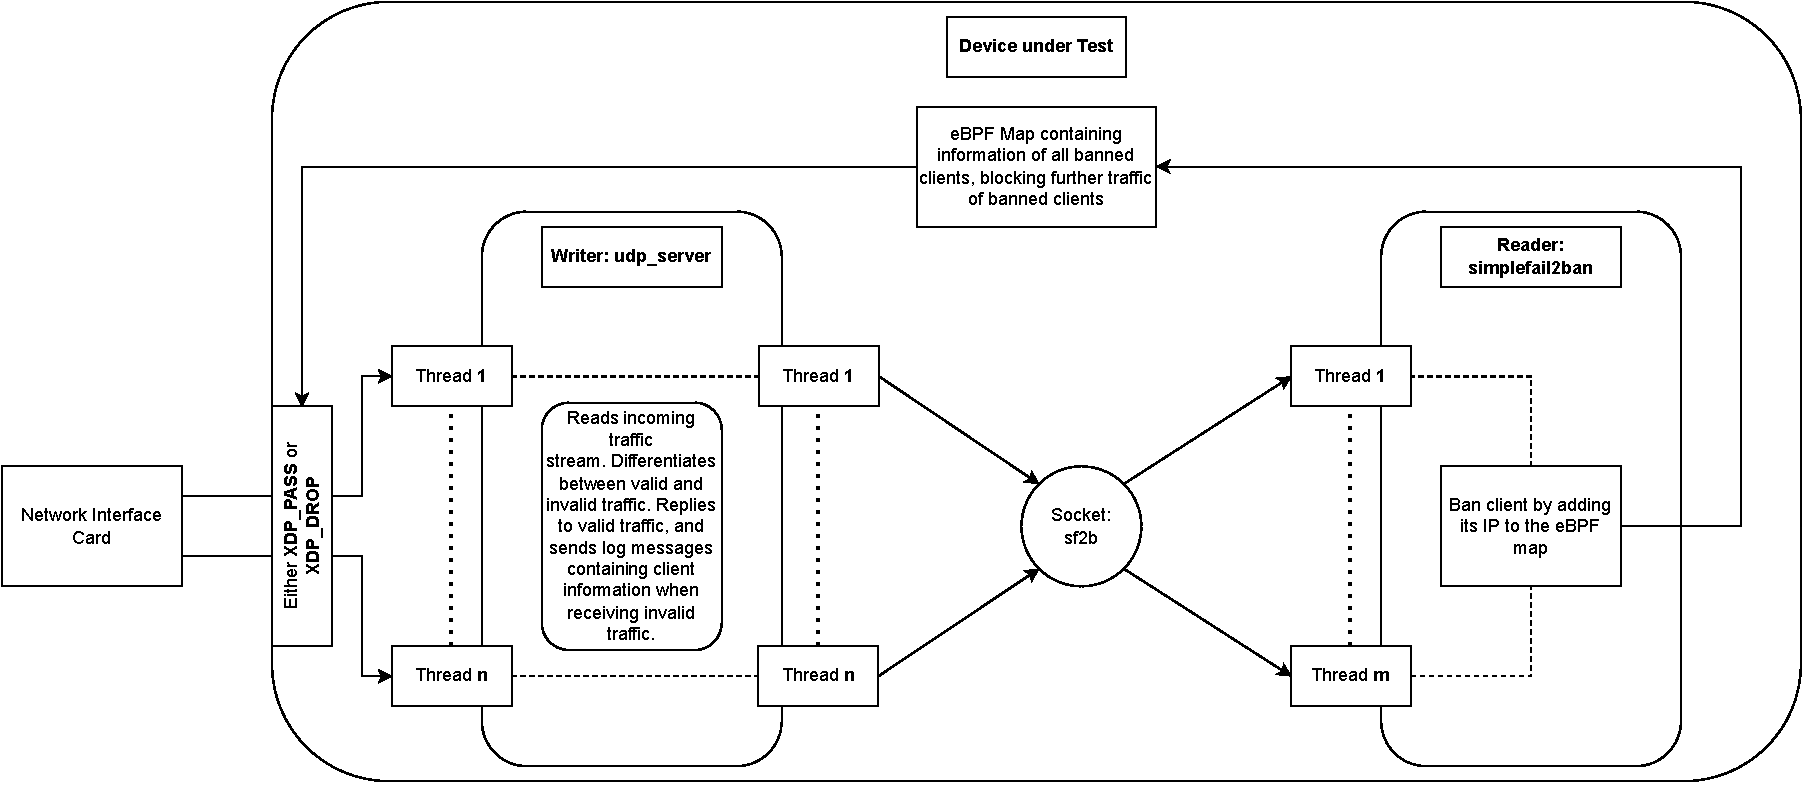
\includegraphics[width=1.2\textwidth]{images/MeasurementArchitecture.pdf}}
    \caption[\ac{DUT} during socket measurements]{
        displays the data flow (left to right) on the \ac{DUT} when enabling sockets as the \ac{IPC} type.
        A packet can either be passed (XDP\_PASS) to the kernel or dropped (XDP\_DROP) before ever reaching the kernel.}
	\label{fig:socket:measurement}
\end{figure}


\subsection{Experiment 2: Simplefail2ban Sockets}
To establish a baseline for the performance of the socket mode, all factors are set to all possible levels in every combination.
The only exception being the possibility of using a second reader process, which will have its own section later.
In total, 25 unique measurements were conducted for this experiment.

\subsection{Experiment 3a: Replication of Simplefail2ban Shared Memory with 2nd Reader}
In order to later compare the socket mode and its option to have a second reader, a baseline measurement needs to be established.
This experiment will be performed with 131068 clients sending invalid data only and no pure IPv4 or IPv6 \ac{IP} stack.
Again, the overwrite feature is enabled while workload stealing is disabled.
The second reader process logs all messages it receives in a log file.
In total, 5 unique measurements were conducted for this experiment.

\subsection{Experiment 3b: Simplefail2ban Sockets with 2nd Reader}
This experiment closely mirrors the experiment 3a.
A total of 131068 clients will send invalid data to the \ac{DUT} with no pure IPv4 or IPv6 \ac{IP} stack.
The shared memory mode inherently supports the possibility of adding a second reader to the shared memory section to read log messages.
There is no such inherent support in the socket mode.
Instead in its current implementation, another read process can be started which will then be assigned its own socket.
This socket will then also receive all log messages.
Consequently, the shared memory mode will likely see a smaller performance loss, since no additional effort is required to send messages to the second reader. 
The second reader process logs all messages it receives in a log file.
In total, 5 unique measurements were conducted for this experiment.

\newpage
\section{Evaluation of Experiments}
The aforementioned experiments can be logically grouped in two categories\@: Baseline measurements and utilization of a second reader.
Baseline measurements are conducted in experiments 1a, 1b and 2, second reader experiments in 3a and 3b.
With 85 performed experiments, a thorough yet not unreasonably long evaluation of each measurement is impossible.
Instead, only especially expressive data will be covered in this section, with any notable or diverging observations being explicitly mentioned.
For full measurement data on all experiments, refer to the repository provided in the sources\cite{git:repoOfThesis}.

\minisec{Meaning of data variables}
In the following section, each graph will be accompanied with an additional table.
This table contains data that is not explicitly expressed otherwise.
A total of six lines are plotted, with two of them belonging to each \ac{IPC} type.
For each \ac{IPC} type (File, Shm, Sock), the total number of packets dropped by the \ac{eBPF} program is denominated via \texttt{XDP\_DROP}.
Similarly, the number of packets passed to the kernel is displayed via \texttt{XDP\_PASS}.
The \texttt{relative drop} represents the percentage of packets dropped relative to the theoretical maximal of dropped packets (represented by \texttt{Best-case drop rate}).
Calculating the relative drop is done with the following formula:
total dropped packets $/ ($experiment duration $*$ invalid traffic rate $-$ number of ban cycles $*$ ban limit $*$ number of malicious clients$)$.
Each ban cycle lasts for 30 seconds.
\texttt{Packets received by udp\_server} lists the number of packets reaching the application udp\_server, while \texttt{Log messages} represents the number of messages sent via the chosen \ac{IPC} type.

\subsection{Baseline measurements}
For this section, data of 75 experiments have been analyzed.

\minisec{Using 65534 clients to send invalid data}
A trend displayed in \ref{fig:data:ipv4:100k:65534} remains prevalent with lower rates of invalid traffic with 65534 clients sending invalid data:
Differences in performance are difficult to spot when graphed.
The table in \ref{fig:data:ipv4:100k:65534} does provide more information.
All \ac{IPC} types perform similarly well in defending the \ac{DoS} attack.

However, one anomaly stands out.
The \texttt{relative drop} of the shared memory \ac{IPC} type is over 100\%.
This happened a total of 21 times over separate measurements, but only when measuring traffic rates of 100k \ac{PPS}.
It is suspected that TRex is unable to provide a reliable stream of packets, but only when starting each measurement call.
Once a steady stream of packets at desired rates has been established, it does remain stable.
Therefore, the number of packets that should be received are higher than the actual incoming traffic rate, resulting in slight inaccuracies when calculating the \texttt{relative drop}.
While not directly apparent at 100k \ac{PPS} due to slight rounding, this discrepancy can be detected by totaling \texttt{XDP\_DROP} and \texttt{XDP\_PASS} up and comparing it to the number of packets that should have theoretically been received.
Unfortunately, this issue is present in all data presented in this thesis and depicts a likely flaw in TRex - not the measurements.

Of note is a stark difference in \ac{CPU} time, with a clearly discernible spike when using the socket \ac{IPC} type, likely cause by extensive context-switches between kernel- and userspace.
All \ac{IPC} types have sent the same number of log messages indicating that, at lower traffic rates, all clients can be banned with the first message they send surpassing the ban limit, regardless of \ac{IPC} type.
This claim is supported by the fact that the log messages coincide with the formula:
number of ban cycles $*$ ban limit $*$ number of malicious clients;
which is the theoretical minimum number of messages needed to successfully ban all clients throughout the duration of the measurement. 
Otherwise, the results are as expected with the file \ac{IPC} type performing worst due to increased latency.

\begin{figure}[!h]
	\centering
	\scriptsize
	\begin{tabular}{c}
    	\centerline{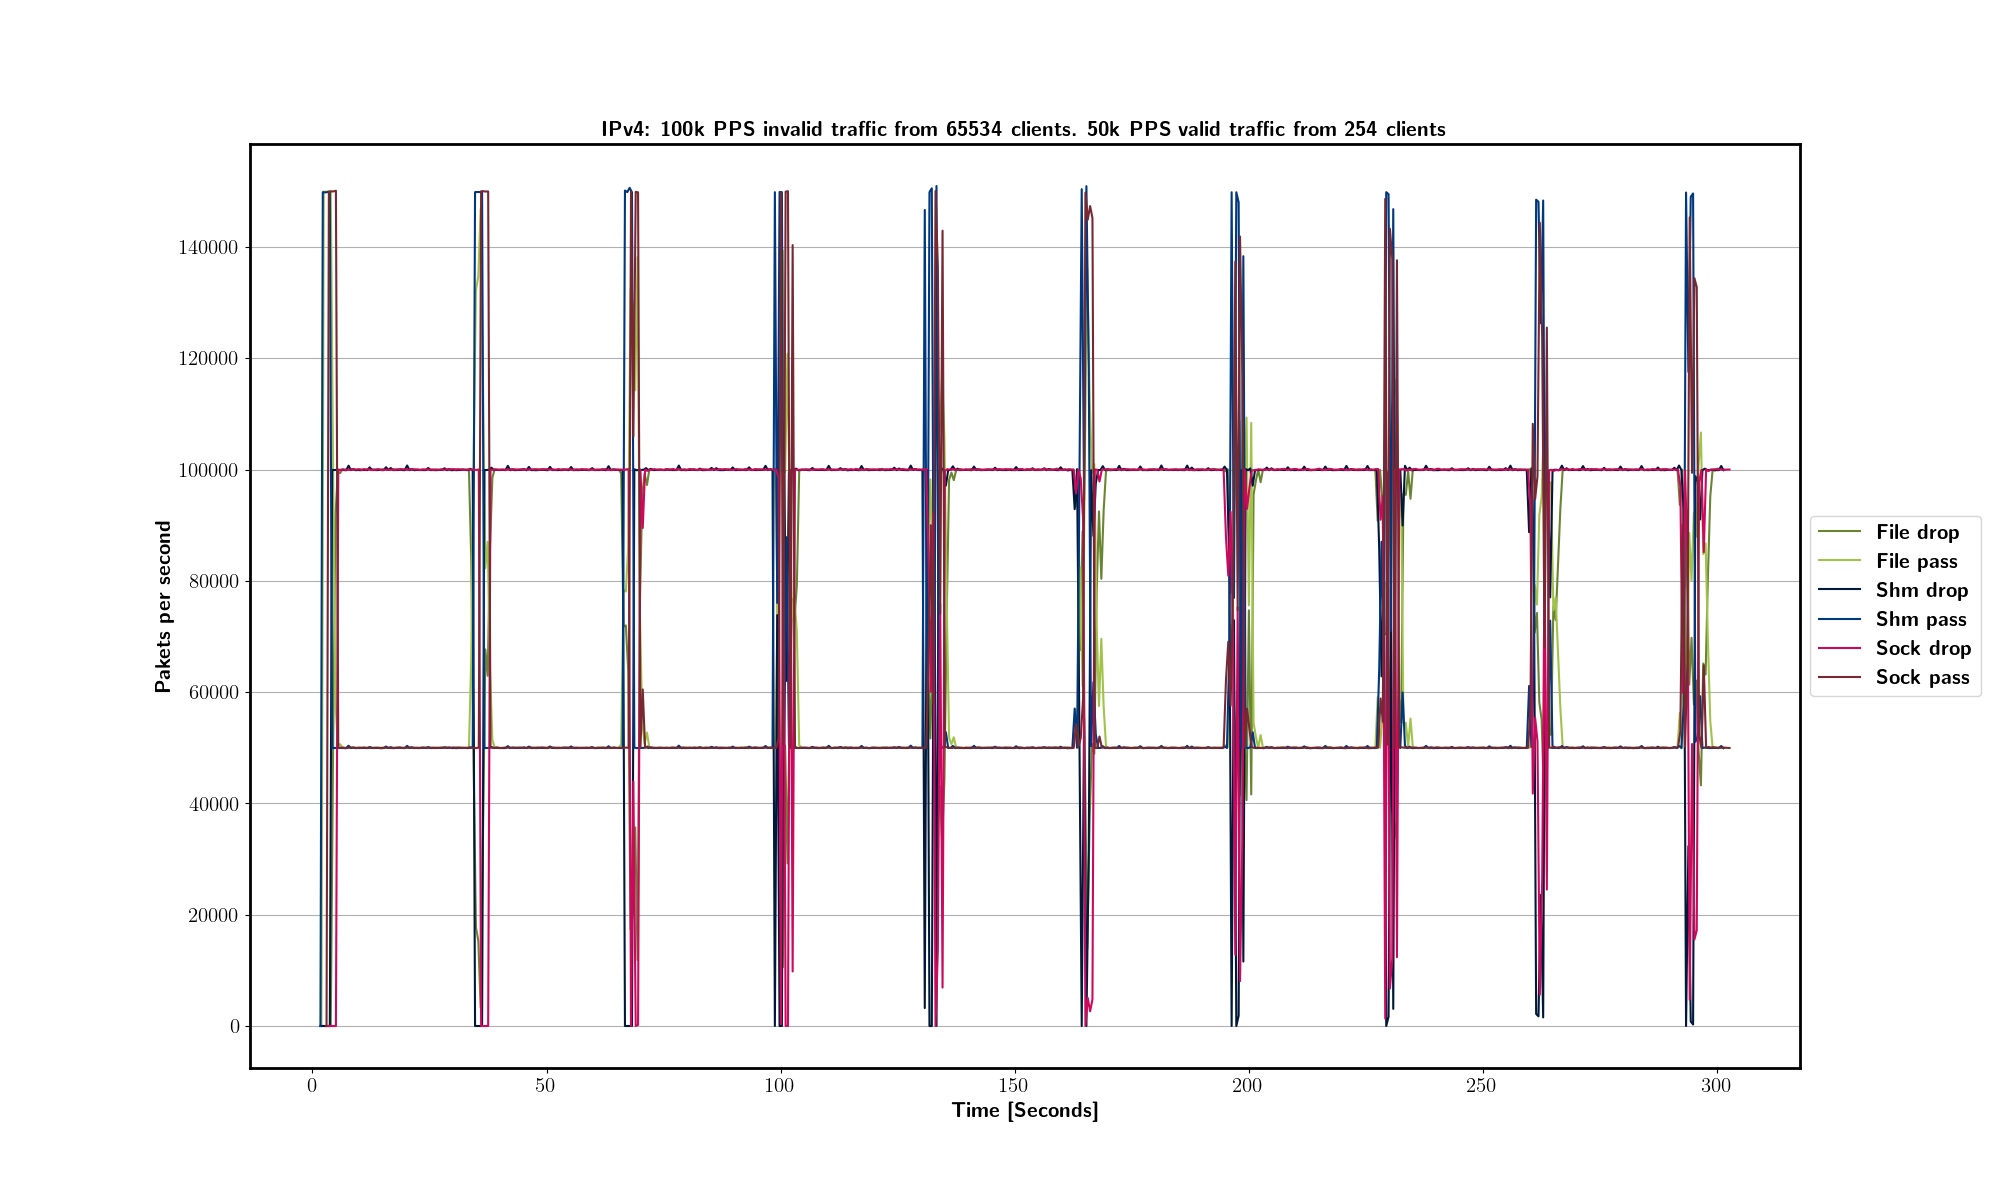
\includegraphics[width=1.2\textwidth]{images/IPv4_100k_65534_1.png}}
	\end{tabular}
	\begin{tabular}{llll}
		\toprule
		\textbf{IPC type} & \textbf{XDP\_DROP [$10^6$]} & \textbf{XDP\_PASS [$10^6$]} & \textbf{Relative drop [\%]} \\ \midrule 
		File & 27,84 & 17,16 & 99,29900071 \\
        Shm & 28,03 & 16,97 & 100,0000036 \\
        Sock & 28,02 & 16,98 & 99,93706566 \\
	\bottomrule
	\end{tabular}
    \begin{tabular}{llll}
		\toprule
		\textbf{IPC type} & \textbf{Packets received by udp\_server [$10^6$]} & \textbf{Log messages [$10^5$]} & \textbf{CPU [seconds]} \\ \midrule 
		File & 16,81 & 19,66 & 04.95 \\
        Shm & 16,97 & 19,66 & 05.94 \\
        Sock & 16,96 & 19,66 & 57.90 \\
	\bottomrule
	\end{tabular}
	\caption[Simplefail2ban, IPv4, 100k \ac{PPS}, 65534 malicious clients]{Total packets sent: 45m. Best-case drop rate: 93,4466\%}
	\label{fig:data:ipv4:100k:65534}
\end{figure}

In \ref{fig:data:ipv4:10m:65534}, the trend of shared memory clearly outperforming other \ac{IPC} types is evident.
Again, differences in plotting the number of dropped and passed packets are to small to be visually decipherable and will be omitted until this changes.
Instead, a clear difference in performance is once again mainly visible in \ac{CPU} time.
The \texttt{relative drop} also reveals that the shared memory \ac{IPC} is performing best, with a lower number of packets being passed to the kernel.
An overall drop in performance measured via \texttt{relative drop} along all \ac{IPC} types was expected.
A generous best-case scenario consists of assuming that all 65534 clients are banned in the same timespan at all incoming traffic rates.
But even then, the inherit latency (even if miniscule) of the \ac{IPS} means that an increase in invalid traffic flow directly correlates with more packets reaching the kernel during each ban cycle.
Therefore, the \texttt{relative drop} rate must inversely correlate with the invalid traffic rate.

\begin{figure}[!h]
	\centering
	\scriptsize
	%\begin{tabular}{c}
    %	\centerline{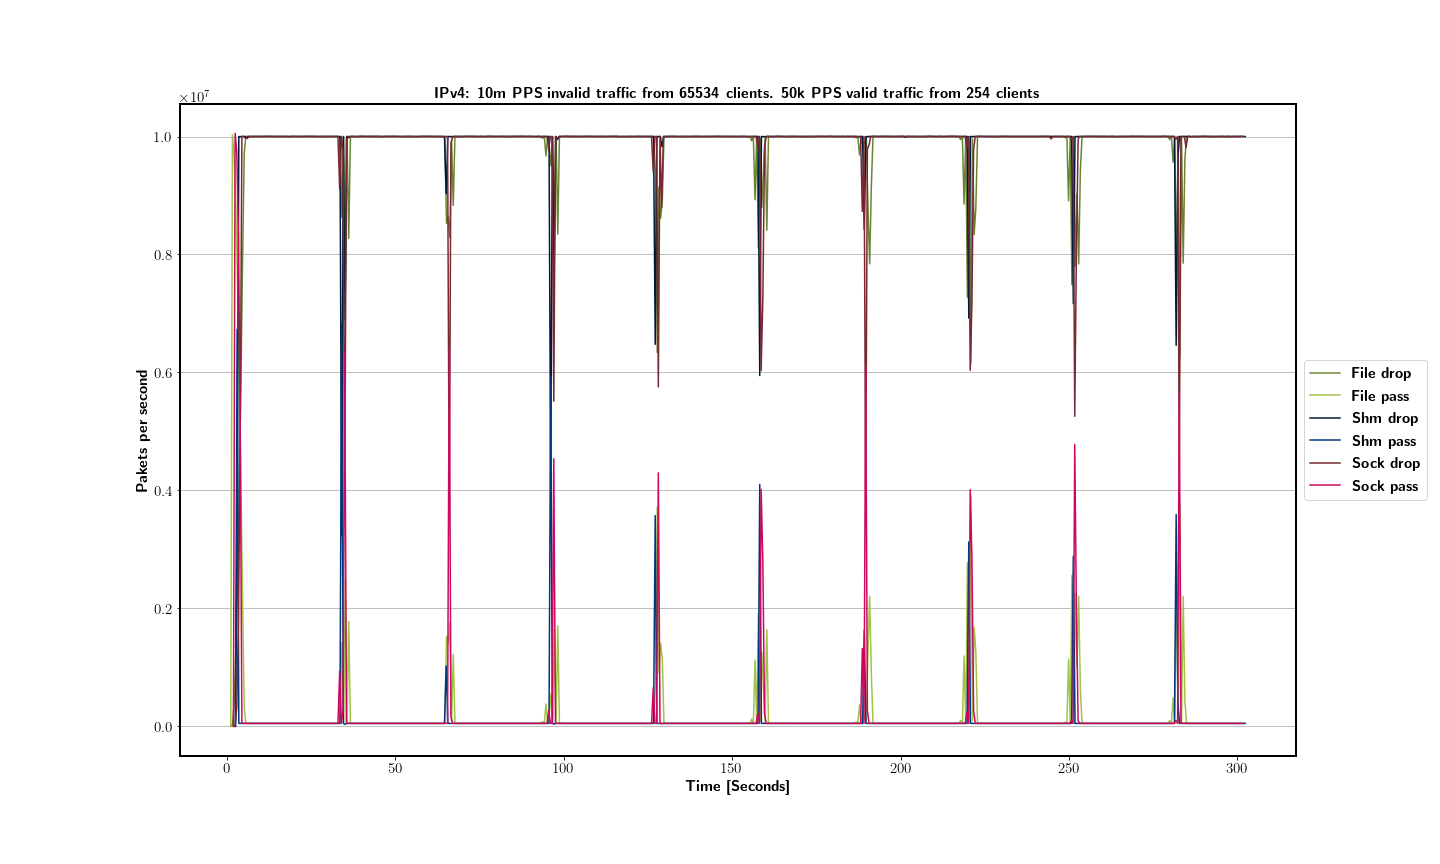
\includegraphics[width=1.2\textwidth]{images/IPv4_10m_65534_1.png}}
	%\end{tabular}
	\begin{tabular}{llll}
		\toprule
		\textbf{IPC type} & \textbf{XDP\_DROP [$10^8$]} & \textbf{XDP\_PASS [$10^6$]} & \textbf{Relative drop [\%]} \\ \midrule 
		File & 29,40 & 75,07 & 98,05973977 \\
        Shm & 29,75 & 37,49 & 99,21848407 \\
        Sock & 29,50 & 61,81 & 98,39458207 \\
	\bottomrule
	\end{tabular}
    \begin{tabular}{llll}
		\toprule
		\textbf{IPC type} & \textbf{Packets received by udp\_server [$10^6$]} & \textbf{Log messages [$10^5$]} & \textbf{CPU [seconds]} \\ \midrule 
		File & 17,51 & 35,10 & 09.69 \\
        Shm & 20,02 & 51,93 & 16.86 \\
        Sock & 17,13 & 25,52 & 76.00 \\
	\bottomrule
	\end{tabular}
	\caption[Simplefail2ban, IPv4, 10m \ac{PPS}, 65534 malicious clients]{Total packets sent: 3015m. Best-case drop rate: 99,934466\%}
	\label{fig:data:ipv4:10m:65534}
\end{figure}

Even with 30m invalid \ac{PPS}, as seen in \ref{fig:data:ipv4:30m:65534}, all \ac{IPC} types successfully defend against the \ac{DoS} attack.
The fact that the file \ac{IPC} type outperforms the socket \ac{IPC} type in terms of \texttt{relative drop} rate is especially noteworthy.
File mode also outperforms shared memory and socket mode on \ac{CPU} usage, which was not expected due to the traditionally high latency of file-based logging approaches.
With the high rate of incoming traffic during a ban cycle, the application udp\_server has to wait on the \ac{IPC} to be able to submit more log messages to Simplefail2ban.
This results in the system being unable to submit a substantial number of packets to udp\_server.
While not explicitly documented in this thesis, these numbers are available in the repository\cite{git:repoOfThesis}.
The difference in packets received by udp\_server and number of passed packets correlates exactly with this observation.
Measuring the number of packets unable to be submitted to udp\_server was done by checking the file \texttt{/proc/net/udp6} on the \ac{DUT}.

A mutual feature of these three measurements is the direct correlation between \texttt{relative drop} rate and number of \texttt{packets received by udp\_server}.
Better performing \ac{IPC} types generally receive more packets despite the fact that they block invalid traffic at an increased rate.
This is explainable through the inability of the system to supply new packets to udp\_server while it is still waiting on the \ac{IPC} architecture to deliver data to the \ac{IPS}.
\ac{IPC} types with lower latency and higher bandwidth can log more messages during the short influx of packets during each ban cycle.
Hence, udp\_server can receive more packets from the system.
These attributes also result in higher \texttt{relative drop} rates, thus causing this observation.

\begin{figure}[!h]
	\centering
	\scriptsize
	%\begin{tabular}{c}
    %	\centerline{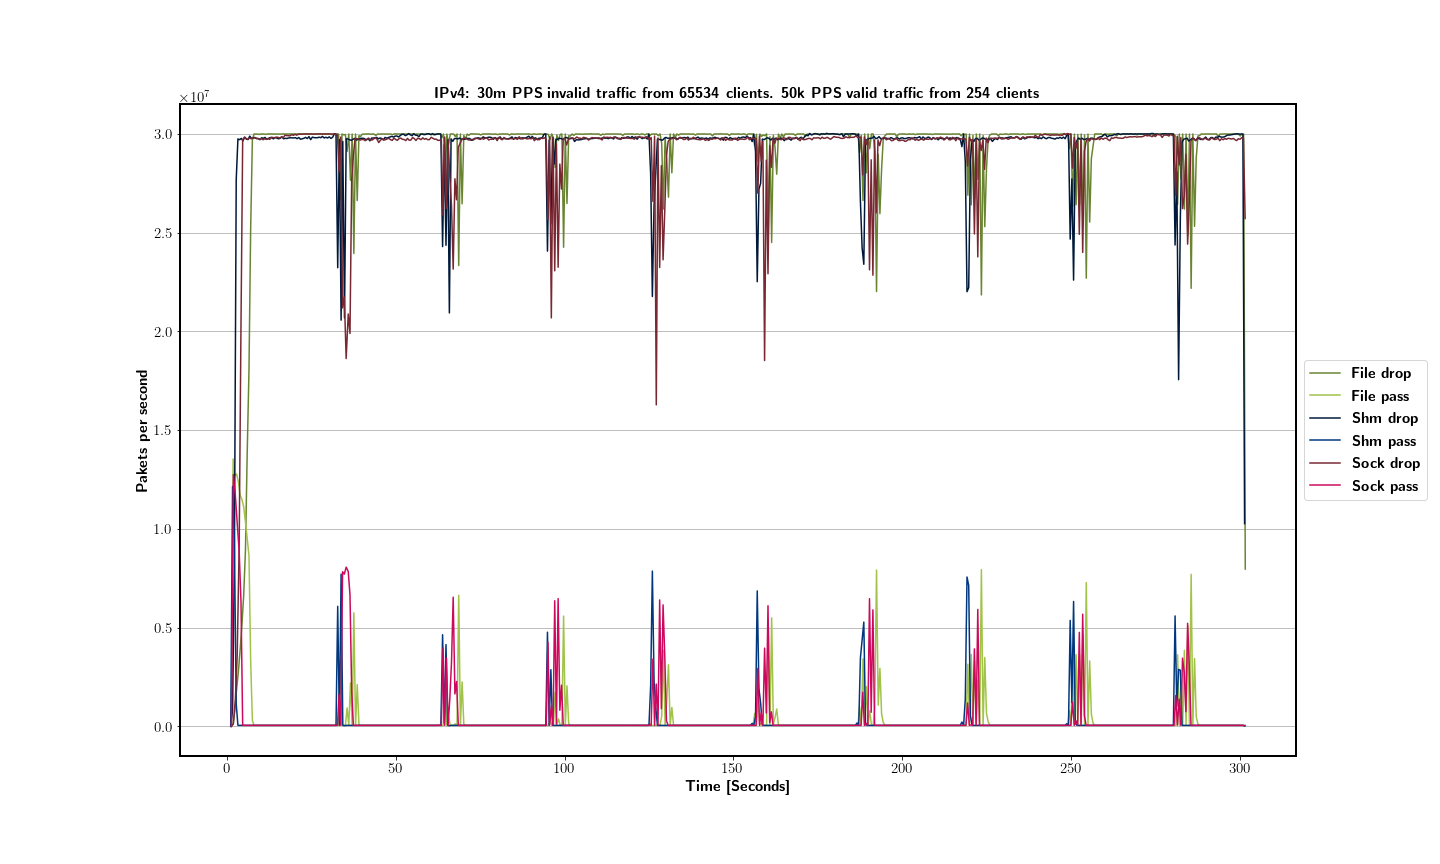
\includegraphics[width=1.2\textwidth]{images/IPv4_30m_65534_1.png}}
	%\end{tabular}
	\begin{tabular}{llll}
		\toprule
		\textbf{IPC type} & \textbf{XDP\_DROP [$10^8$]} & \textbf{XDP\_PASS [$10^6$]} & \textbf{Relative drop [\%]}\\ \midrule 
		File & 87,75 & 159,82 & 97,52375345 \\
        Shm & 88,30 & 87,23 & 98,13105047 \\
        Sock & 87,45 & 139,42 & 97,18179422 \\
	\bottomrule
	\end{tabular}
    \begin{tabular}{llll}
		\toprule
		\textbf{IPC type} & \textbf{Packets received by udp\_server [$10^6$]} & \textbf{Log messages [$10^5$]} & \textbf{CPU [seconds]} \\ \midrule 
		File & 17,48 & 40,72 & 16.55 \\
        Shm & 21,39 & 69,92 & 39.08 \\
        Sock & 16,92 & 31,62 & 138.85 \\
	\bottomrule
	\end{tabular}
	\caption[Simplefail2ban, IPv4, 30m \ac{PPS}, 65534 malicious clients]{Total packets sent: 9015m. Best-case drop rate: 99,97815533\%}
	\label{fig:data:ipv4:30m:65534}
\end{figure}

Figure \ref{fig:data:ipv6:30m:65534} displays \ac{IPC} types under 30m invalid \ac{PPS} from 65534 different clients using IPv6 addresses in contrast to the previously used IPv4 addresses.
Usage of different \ac{IP} stacks had little impact on the overall results of this thesis, which is why lower traffic rates for IPv6 are omitted.

As expected, the file \ac{IPC} type performed worst, with shared memory performing best.
However, contradicting expectations, the socket and shared memory \ac{IPC} types performed better when dealing with IPv6 instead of IPv4 addresses.
This is surprising since no changes in general behavior are expected in either udp\_server or Simplefail2ban with one exception: The \ac{Regex} matching feature.
In theory, IPv6 banning should be less performant than using IPv4, because IPv6 addresses are longer than IPv4 addresses.
Reading these addresses out of the log messages received by Simplefail2ban using the \ac{Regex} matching feature should require more time.
This idea is supported by the increase in \ac{CPU} time across all \ac{IPC} types compared to figure \ref{fig:data:ipv4:30m:65534} using IPv4.
However, an increase in performance can be measured in almost all experiments using IPv6 instead of IPv4.
What exactly causes this abnormality is unclear.

\begin{figure}[!h]
	\centering
	\scriptsize
	%\begin{tabular}{c}
    %	\centerline{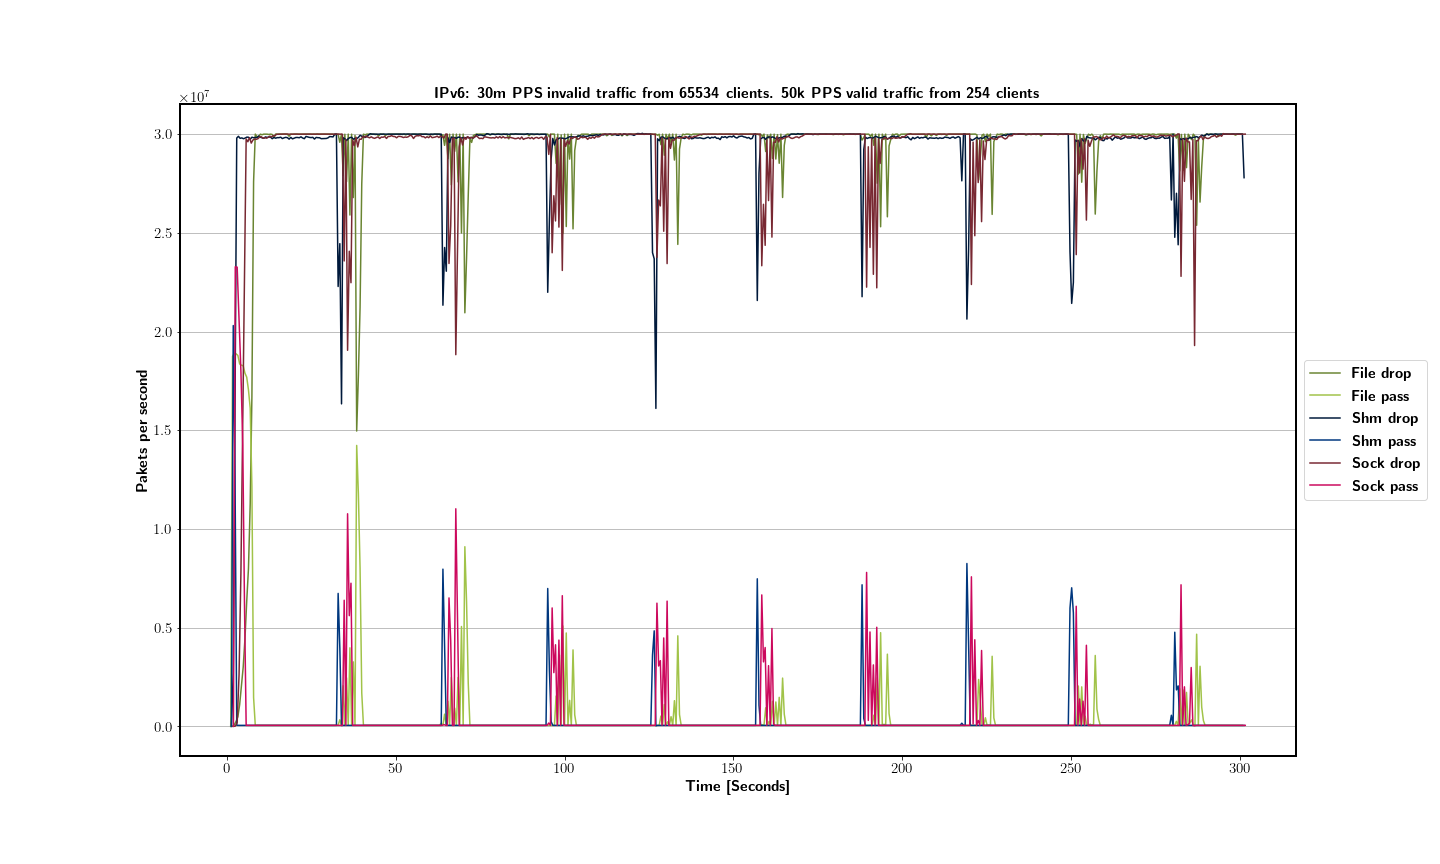
\includegraphics[width=1.2\textwidth]{images/IPv6_30m_65534_1.png}}
	%\end{tabular}
	\begin{tabular}{llll}
		\toprule
		\textbf{IPC type} & \textbf{XDP\_DROP [$10^8$]} & \textbf{XDP\_PASS [$10^6$]} & \textbf{Relative drop [\%]} \\ \midrule 
		File & 87,41 & 211,05 & 97,14091697 \\
        Shm & 88,63 & 85,55 & 98,50239609 \\
        Sock & 87,77 & 170,03 & 97,54838057 \\
	\bottomrule
	\end{tabular}
    \begin{tabular}{llll}
		\toprule
		\textbf{IPC type} & \textbf{Packets received by udp\_server [$10^6$]} & \textbf{Log messages [$10^5$]} & \textbf{CPU [seconds]} \\ \midrule 
		File & 17,20 & 38,73 & 22.51 \\
        Shm & 21,79 & 72,38 & 46.03 \\
        Sock & 16,92 & 30,04 & 149.69 \\
	\bottomrule
	\end{tabular}
	\caption[Simplefail2ban, IPv6, 30m \ac{PPS}, 65534 malicious clients]{Total packets sent: 9015m. Best-case drop rate: 99,97815533\%}
	\label{fig:data:ipv6:30m:65534}
\end{figure}

\minisec{Using 131068 clients to send invalid data}
When using 131068 clients to send invalid data, changes in performance become visible when plotted.
Figure \ref{fig:data:ipv4:100k:131068} displays only 100k invalid \ac{PPS}, yet the file \ac{IPC} type struggles to quickly ban all clients.
In contrast, both socket and shared memory seem to perform quite similarly across all statistics except for \ac{CPU} time.
Here, the socket \ac{IPC} type occupies the \ac{CPU} almost ten times longer than shared memory, again likely due to extensive context-switches between kernel- and userspace.

\begin{figure}[!h]
	\centering
	\scriptsize
	\begin{tabular}{c}
    	\centerline{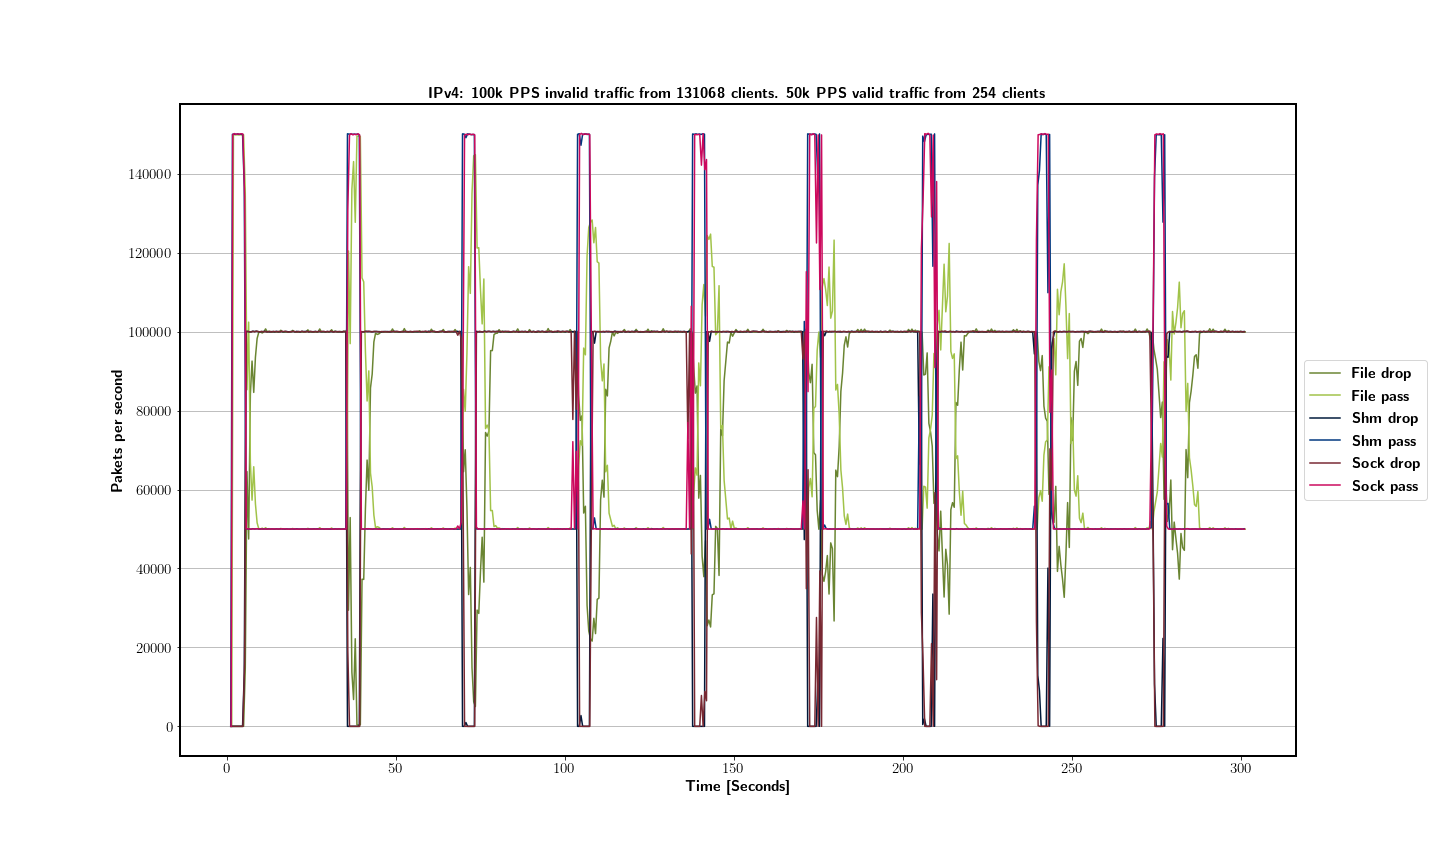
\includegraphics[width=1.2\textwidth]{images/IPv4_100k_131068_1.png}}
	\end{tabular}
	\begin{tabular}{llll}
		\toprule
		\textbf{IPC type} & \textbf{XDP\_DROP [$10^6$]} & \textbf{XDP\_PASS [$10^6$]} & \textbf{Relative drop [\%]} \\ \midrule 
		File & 25,99 & 19,01 & 99,69409958 \\
        Shm & 26,46 & 18,54 & 101,5083842 \\
        Sock & 26,44 & 18,56 & 101,4395334 \\
	\bottomrule
	\end{tabular}
    \begin{tabular}{llll}
		\toprule
		\textbf{IPC type} & \textbf{Packets received by udp\_server [$10^6$]} & \textbf{Log messages [$10^5$]} & \textbf{CPU [seconds]} \\ \midrule 
		File & 18,16 & 35,39 & 08.34 \\
        Shm & 18,54 & 35,39 & 10.14 \\
        Sock & 18,53 & 35,39 & 100.40 \\
	\bottomrule
	\end{tabular}
	\caption[Simplefail2ban, IPv4, 100k \ac{PPS}, 131068 malicious clients]{Total packets sent: 45m. Best-case drop rate: 86,8932\%}
	\label{fig:data:ipv4:100k:131068}
\end{figure}

At invalid traffic rates of 10m \ac{PPS}, displayed in figure \ref{fig:data:ipv4:10m:131068}, drastic changes are noticeable.
Firstly, shared memory does outperform both the socket and file \ac{IPC} type in \texttt{relative drop} rate.
Also, the latency of each \ac{IPC} type is clearly visible in the provided graph via their drasticly shifted spike of dropped packets each ban cycle.
The shared memory \ac{IPC} type both starts and ends its ban cycles before the socket and file \ac{IPC} type.
Unexpectedly, the socket \ac{IPC} type still outperforms the file \ac{IPC} type in \texttt{relative drop} rate.
A general delay of each ban cycle is visible too.
The second to last ban cycle, which should start at 240 seconds, starts late at about 250 seconds.
This delay is present in all \ac{IPC} types. 
It is likely caused by the unbanning thread of Simplefail2ban having to handle 131068 clients, resulting in them being banned, on average, slightly longer than the intended 30 seconds.

\begin{figure}[!h]
	\centering
	\scriptsize
	\begin{tabular}{c}
    	\centerline{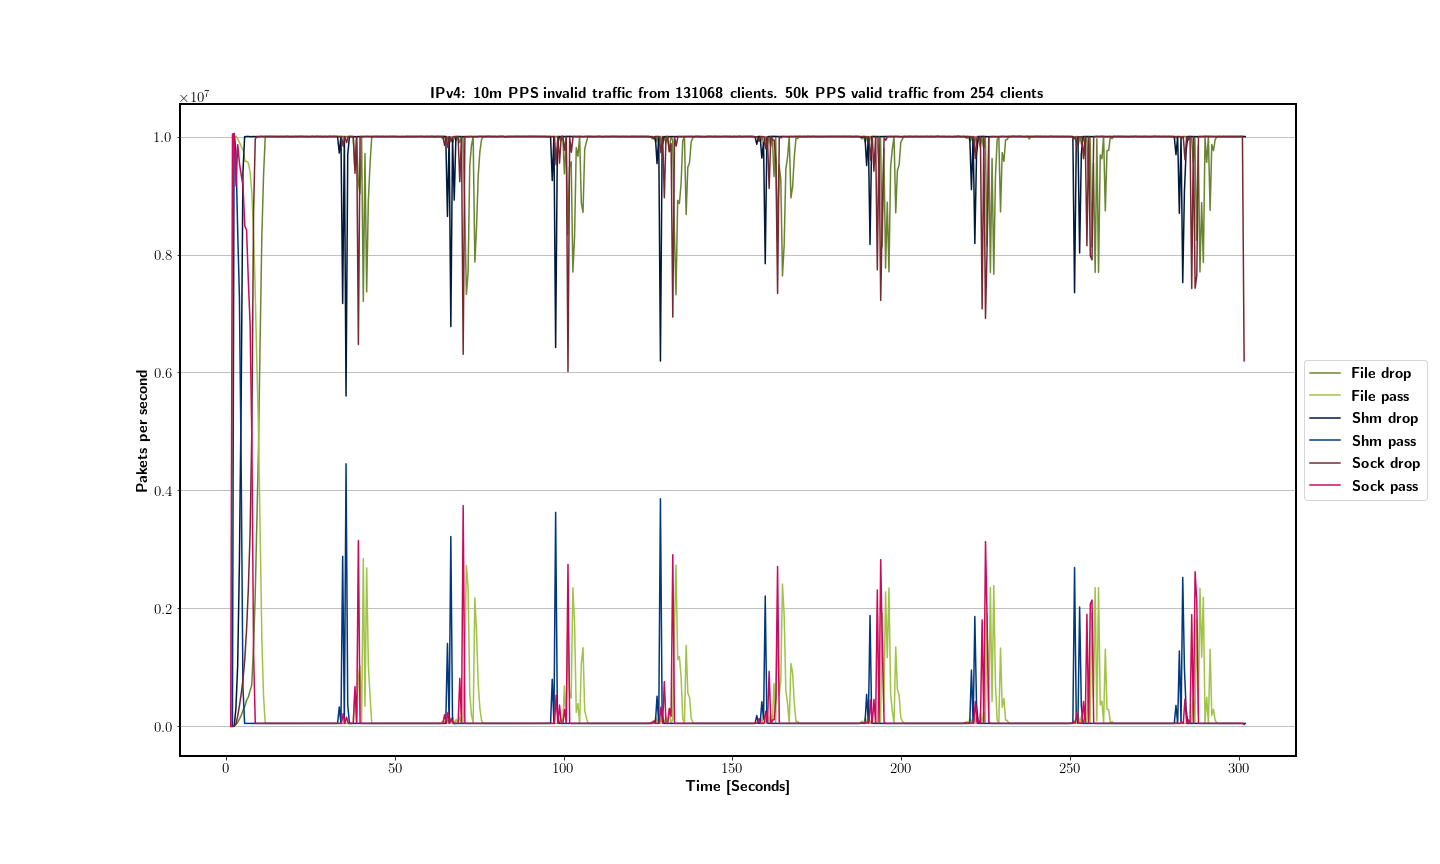
\includegraphics[width=1.2\textwidth]{images/IPv4_10m_131068_1.png}}
	\end{tabular}
	\begin{tabular}{llll}
		\toprule
		\textbf{IPC type} & \textbf{XDP\_DROP [$10^8$]} & \textbf{XDP\_PASS [$10^6$]} & \textbf{Relative drop [\%]} \\ \midrule 
		File & 28,77 & 136,15 & 96,03486581 \\
        Shm & 29,54 & 58,36 & 98,60515631 \\
        Sock & 29,16 & 95,52 & 97,33669129 \\
	\bottomrule
	\end{tabular}
    \begin{tabular}{llll}
		\toprule
		\textbf{IPC type} & \textbf{Packets received by udp\_server [$10^6$]} & \textbf{Log messages [$10^5$]} & \textbf{CPU [seconds]} \\ \midrule 
		File & 19,31 & 63,90 & 19.39 \\
        Shm & 25,40 & 107,54 & 29.47 \\
        Sock & 19,02 & 47,67 & 133.54 \\
	\bottomrule
	\end{tabular}
	\caption[Simplefail2ban, IPv4, 10m \ac{PPS}, 131068 malicious clients]{Total packets sent: 3015m. Best-case drop rate: 99,868932\%}
	\label{fig:data:ipv4:10m:131068}
\end{figure}

At 30m invalid \ac{PPS}, seen in figure \ref{fig:data:ipv4:30m:131068}, the file \ac{IPC} type starts and finishes its ban cycles later than other \ac{IPC} types.
While the shared memory and socket \ac{IPC} type start almost simultaneously, sockets require longer to finish a full ban cycle.
Differences in \ac{CPU} time are prominent, with the socket \ac{IPC} performing worst and file \ac{IPC} performing best according to the \texttt{relative drop} rate.
A general trend found in all measurements presented is the low throughput of the socket \ac{IPC} type.
Here, it is especially pronounced with the shared memory \ac{IPC} type managing to transmit almost double the amount of \texttt{log messages}.

\begin{figure}[!h]
	\centering
	\scriptsize
	\begin{tabular}{c}
    	\centerline{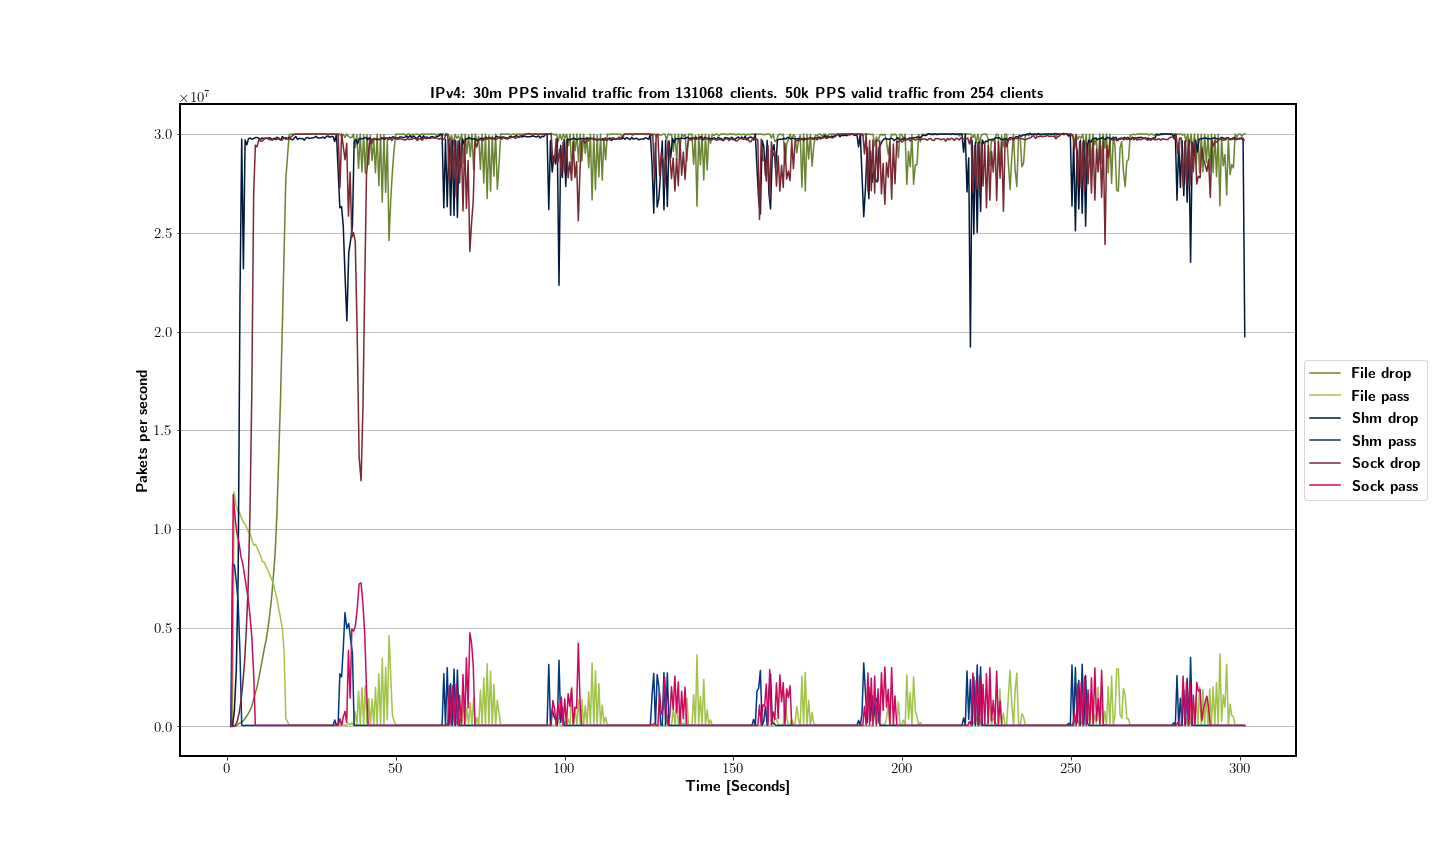
\includegraphics[width=1.2\textwidth]{images/IPv4_30m_131068_2.png}}
	\end{tabular}
	\begin{tabular}{llll}
		\toprule
		\textbf{IPC type} & \textbf{XDP\_DROP [$10^8$]} & \textbf{XDP\_PASS [$10^6$]} & \textbf{Relative drop [\%]} \\ \midrule 
		File & 85,02 & 238,30 & 94,51036756 \\
        Shm & 87,57 & 104,14 & 97,33826458 \\
        Sock & 86,12 & 180,89 & 95,73084169 \\
	\bottomrule
	\end{tabular}
    \begin{tabular}{llll}
		\toprule
		\textbf{IPC type} & \textbf{Packets received by udp\_server [$10^6$]} & \textbf{Log messages [$10^5$]} & \textbf{CPU [seconds]} \\ \midrule 
		File & 18,04 & 74,39 & 38.99 \\
        Shm & 25,32 & 115,04 & 71.92 \\
        Sock & 18,33 & 59,26 & 323.02 \\
	\bottomrule
	\end{tabular}
	\caption[Simplefail2ban, IPv4, 30m \ac{PPS}, 131068 malicious clients]{Total packets sent: 9015m. Best-case drop rate: 99,95631067\%}
	\label{fig:data:ipv4:30m:131068}
\end{figure}

Switching to IPv6 at a rate of 30m invalid \ac{PPS} does not yield any fundamentally different results: \ref{fig:data:ipv6:30m:131068}.
Again, performance of all \ac{IPC} types improves slightly, still with no known cause.
Shared memory performs best, with the file \ac{IPC} type performing worst.
The direct correlation between \texttt{relative drop} rate and \texttt{packets received by udp\_server} is also still present.

\begin{figure}[!h]
	\centering
	\scriptsize
	%\begin{tabular}{c}
    %	\centerline{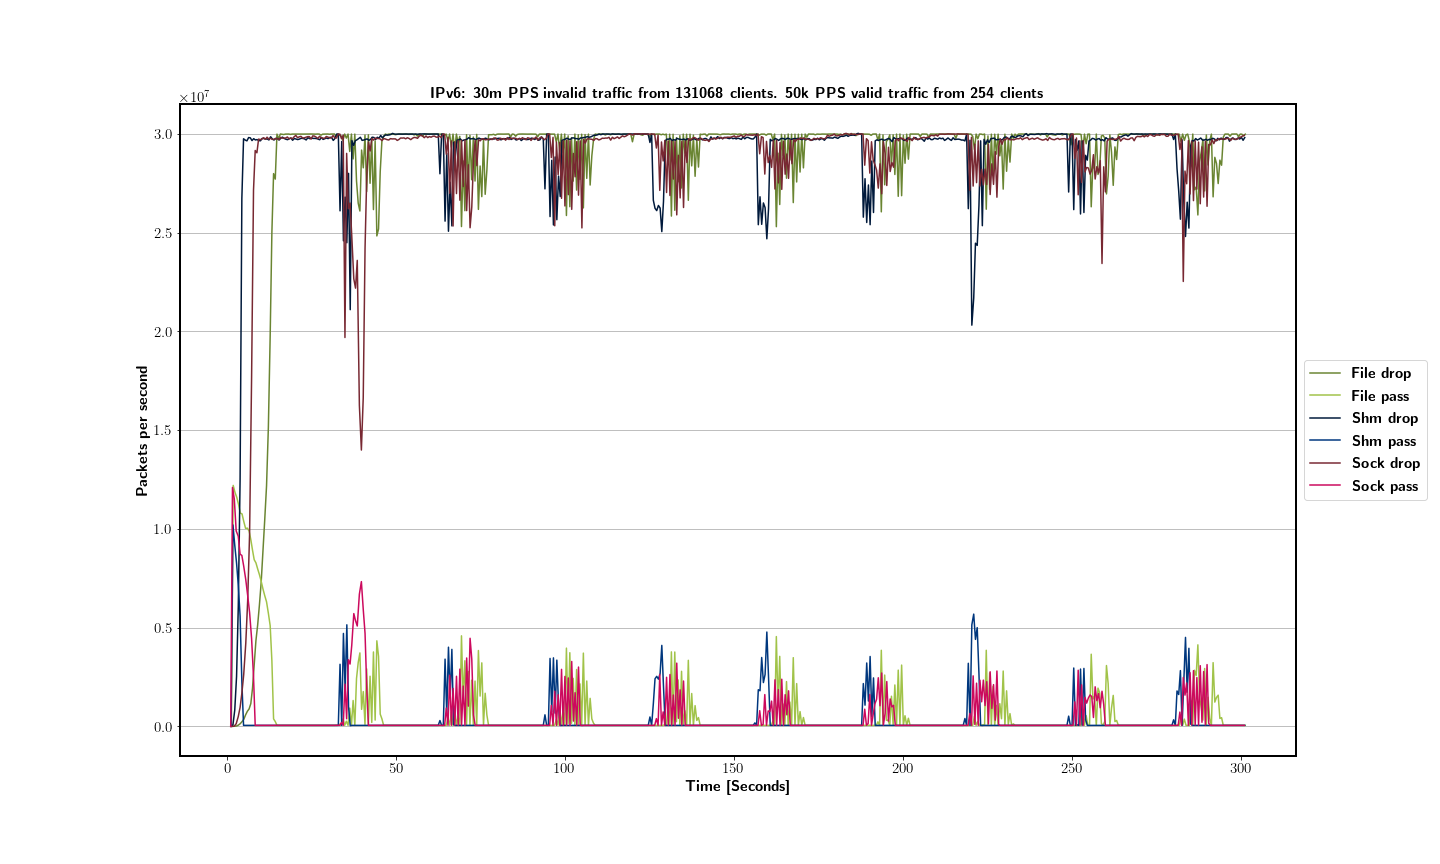
\includegraphics[width=1.2\textwidth]{images/IPv6_30m_131068_1.png}}
	%\end{tabular}
	\begin{tabular}{llll}
		\toprule
		\textbf{IPC type} & \textbf{XDP\_DROP [$10^8$]} & \textbf{XDP\_PASS [$10^6$]} & \textbf{Relative drop [\%]} \\ \midrule 
		File & 85,73 & 228,07 & 95,29278185 \\
        Shm & 87,60 & 109,08 & 97,37706621 \\
        Sock & 86,21 & 177,33 & 95,82614459 \\
	\bottomrule
	\end{tabular}
    \begin{tabular}{llll}
		\toprule
		\textbf{IPC type} & \textbf{Packets received by udp\_server [$10^6$]} & \textbf{Log messages [$10^5$]} & \textbf{CPU [seconds]} \\ \midrule 
		File & 17,90 & 69,14 & 38.41 \\
        Shm & 25,08 & 111,45 & 74.71 \\
        Sock & 18,67 & 61,84 & 317.37 \\
	\bottomrule
	\end{tabular}
	\caption[Simplefail2ban, IPv6, 30m \ac{PPS}, 131068 malicious clients]{Total packets sent: 9015m. Best-case drop rate: 99,95631067\%}
	\label{fig:data:ipv6:30m:131068}
\end{figure}

When using a mixed \ac{IP} stack, two streams of invalid data were configured in TRex: One being IPv4, the other being IPv6.
Both streams were producing exactly 50\% of the invalid traffic and consisted out of 65534 clients each.
Naturally, no single client sent both IPv4 and IPv6 packets.
The most expressive measurement is displayed in \ref{fig:data:ipv4v6:30m:131068} with 30m invalid \ac{PPS}.
Expectations were that the \texttt{relative drop} rate for all \ac{IPC} types would land firmly between the equivalent measurements using IPv4 and IPv6.
However, this is not the case.
The figure \ref{fig:data:ipv4v6:30m:131068} does not display this property.
In fact, no other measurements using a mixed \ac{IP} stack definitively exhibit this property.
Here, in figure \ref{fig:data:ipv4v6:30m:131068}, the shared memory and socket \ac{IPC} types outperform the measurement utilizing pure IPv6 displayed in \ref{fig:data:ipv6:30m:131068}.
Though, most measurements still outperform their pure IPv4 counterpart at a minimum.
But performance regarding their pure IPv6 counterpart is not definitive, the variance between measurements is too severe.

\begin{figure}[!h]
	\centering
	\scriptsize
	%\begin{tabular}{c}
    %	\centerline{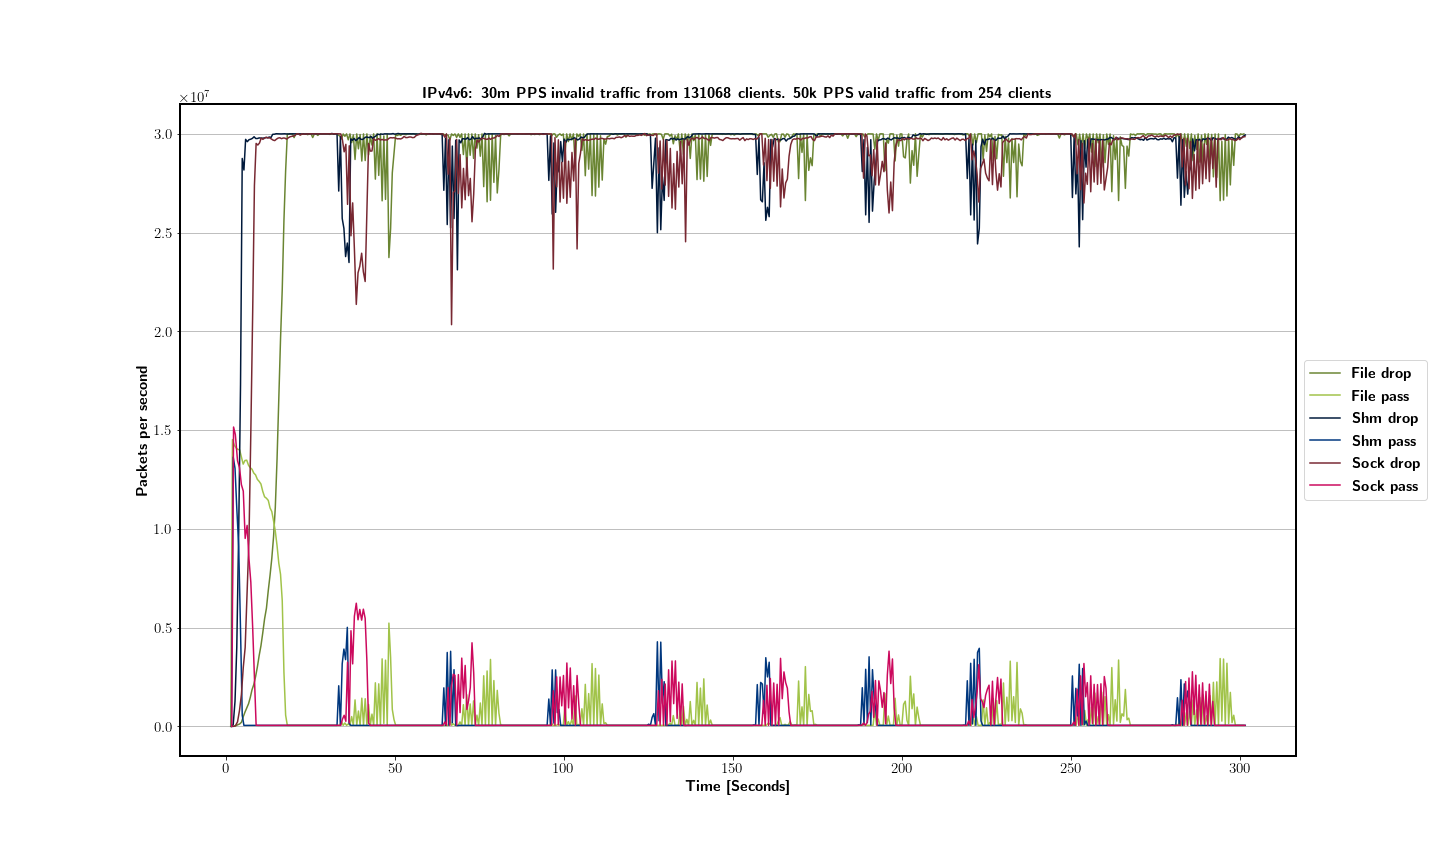
\includegraphics[width=1.2\textwidth]{images/IPv4v6_30m_131068_2.png}}
	%\end{tabular}
	\begin{tabular}{llll}
		\toprule
		\textbf{IPC type} & \textbf{XDP\_DROP [$10^8$]} & \textbf{XDP\_PASS [$10^6$]} & \textbf{Relative drop [\%]} \\ \midrule 
		File & 85,12 & 286,15 & 94,61335186 \\
        Shm & 88,02 & 105,83 & 97,84149307 \\
        Sock & 86,30 & 212,81 & 95,93428297 \\
	\bottomrule
	\end{tabular}
    \begin{tabular}{llll}
		\toprule
		\textbf{IPC type} & \textbf{Packets received by udp\_server [$10^6$]} & \textbf{Log messages [$10^5$]} & \textbf{CPU [seconds]} \\ \midrule 
		File & 17,69 & 70,65 & 47.15 \\
        Shm & 25,13 & 111,62 & 94.64 \\
        Sock & 18,00 & 59,85 & 353.34 \\
	\bottomrule
	\end{tabular}
	\caption[Simplefail2ban, IPv4v6, 30m \ac{PPS}, 131068 malicious clients]{Total packets sent: 9015m. Best-case drop rate: 99,95631067\%}
	\label{fig:data:ipv4v6:30m:131068}
\end{figure}

\subsection{2nd reader measurements}
Initially, data of 10 experiments have been analyzed for this section.
At 100k invalid \ac{PPS}, performance of both the shared memory and socket \ac{IPC} types was almost identical.
The only exception is the \ac{CPU} time in which the socket \ac{IPC} performed up to six times worse than shared memory.
The results become interesting when increasing invalid traffic rate to 1m \ac{PPS}, a seen in figure \ref{fig:data:ipv4v6:1m:131068:2nd}.
The graph displays a clear delay between the ban cycles of the shared memory and socket \ac{IPC} types.
Still, both modes are able to supply both the \ac{IPS} Simplefail2ban and a slower reader process with data while defending against the \ac{DoS} attack.
Again, \ac{CPU} time of the socket \ac{IPC} type is significantly higher than its shared memory counterpart.
The \texttt{relative drop} rate is also worse by about 2 percent (equal to 6,3M more packets reaching the kernel over the duration of the measurement), with fewer messages logged.

\begin{figure}[!h]
	\centering
	\scriptsize
	\begin{tabular}{c}
    	\centerline{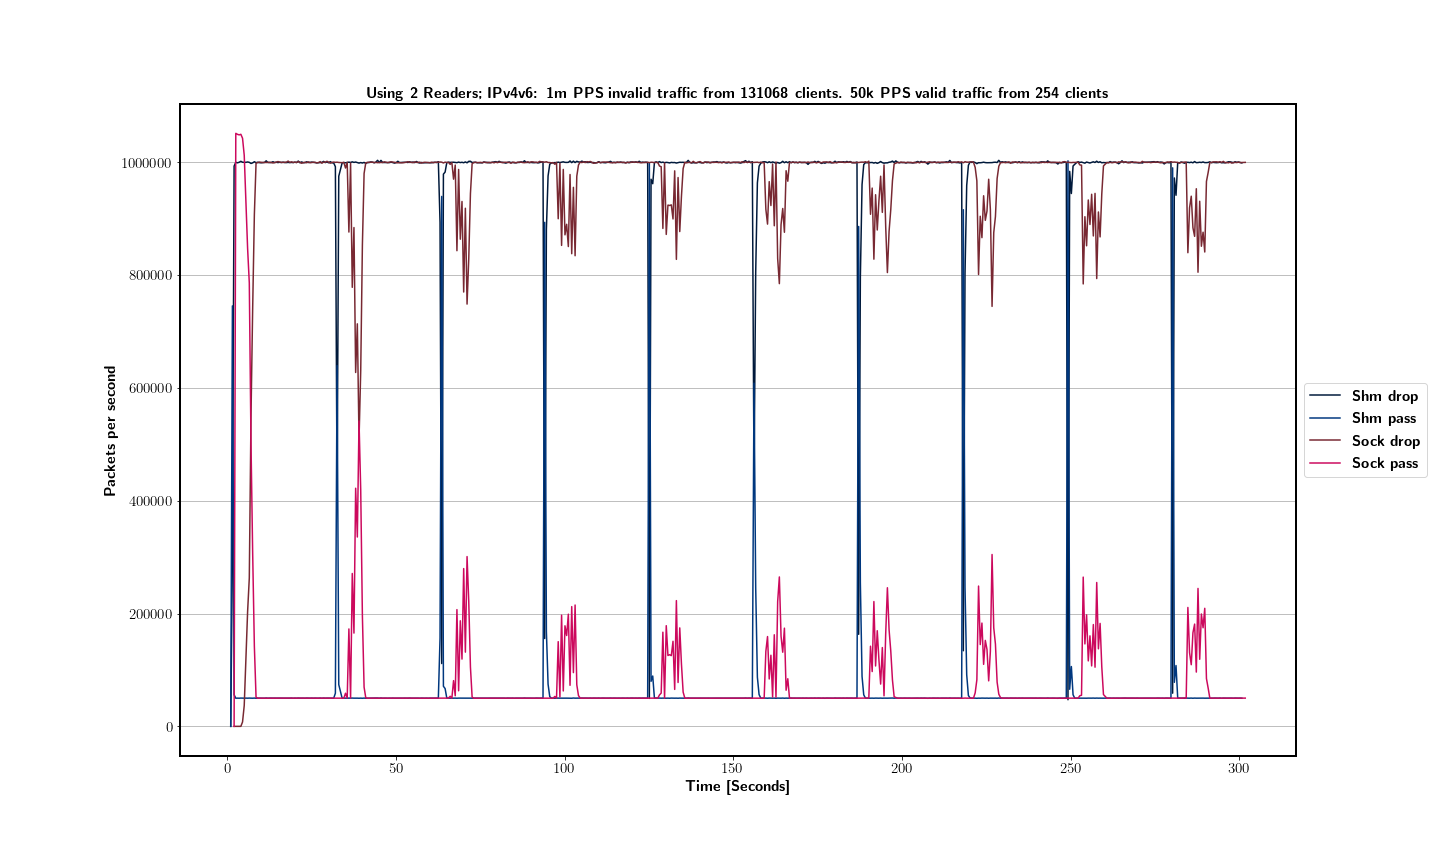
\includegraphics[width=1.2\textwidth]{images/IPv4v6_1m_2ndReader_1.png}}
	\end{tabular}
	\begin{tabular}{llll}
		\toprule
		\textbf{IPC type} & \textbf{XDP\_DROP [$10^7$]} & \textbf{XDP\_PASS [$10^6$]} & \textbf{Relative drop [\%]} \\ \midrule 
		Shm & 29,53 & 19,75 & 99,72283593 \\
        Sock & 28,91 & 25,94 & 97,6334018 \\
	\bottomrule
	\end{tabular}
    \begin{tabular}{llll}
		\toprule
		\textbf{IPC type} & \textbf{Packets received by udp\_server [$10^6$]} & \textbf{Log messages [$10^5$]} & \textbf{CPU [seconds]} \\ \midrule 
		Shm & 19,48 & 44,91 & 17.76 \\
        Sock & 18,29 & 41,47 & 80.82 \\
	\bottomrule
	\end{tabular}
	\caption[Simplefail2ban with 2nd Reader, IPv4v6, 1m \ac{PPS}, 131068 malicious clients]{Total packets sent: 315m. Best-case drop rate: 98,68932\%}
	\label{fig:data:ipv4v6:1m:131068:2nd}
\end{figure}

Figure \ref{fig:data:ipv4v6:20m:131068:2nd} shows data measured with 20m invalid \ac{PPS}.
The socket \ac{IPC} type struggles to supply both the \ac{IPS} and the second reader with \texttt{log messages}, having logged less data than the shared memory \ac{IPC} type.
The graph also displays this inability to keep up with incoming traffic during the first two ban cycles.
While shared memory was able to fully ban all malicious client in just one 30 second ban cycle, the socket mode is not.
Given enough time, the socket \ac{IPC} type is able to recover and successfully defend against the \ac{DoS} attack.

\begin{figure}[!h]
	\centering
	\scriptsize
	\begin{tabular}{c}
    	\centerline{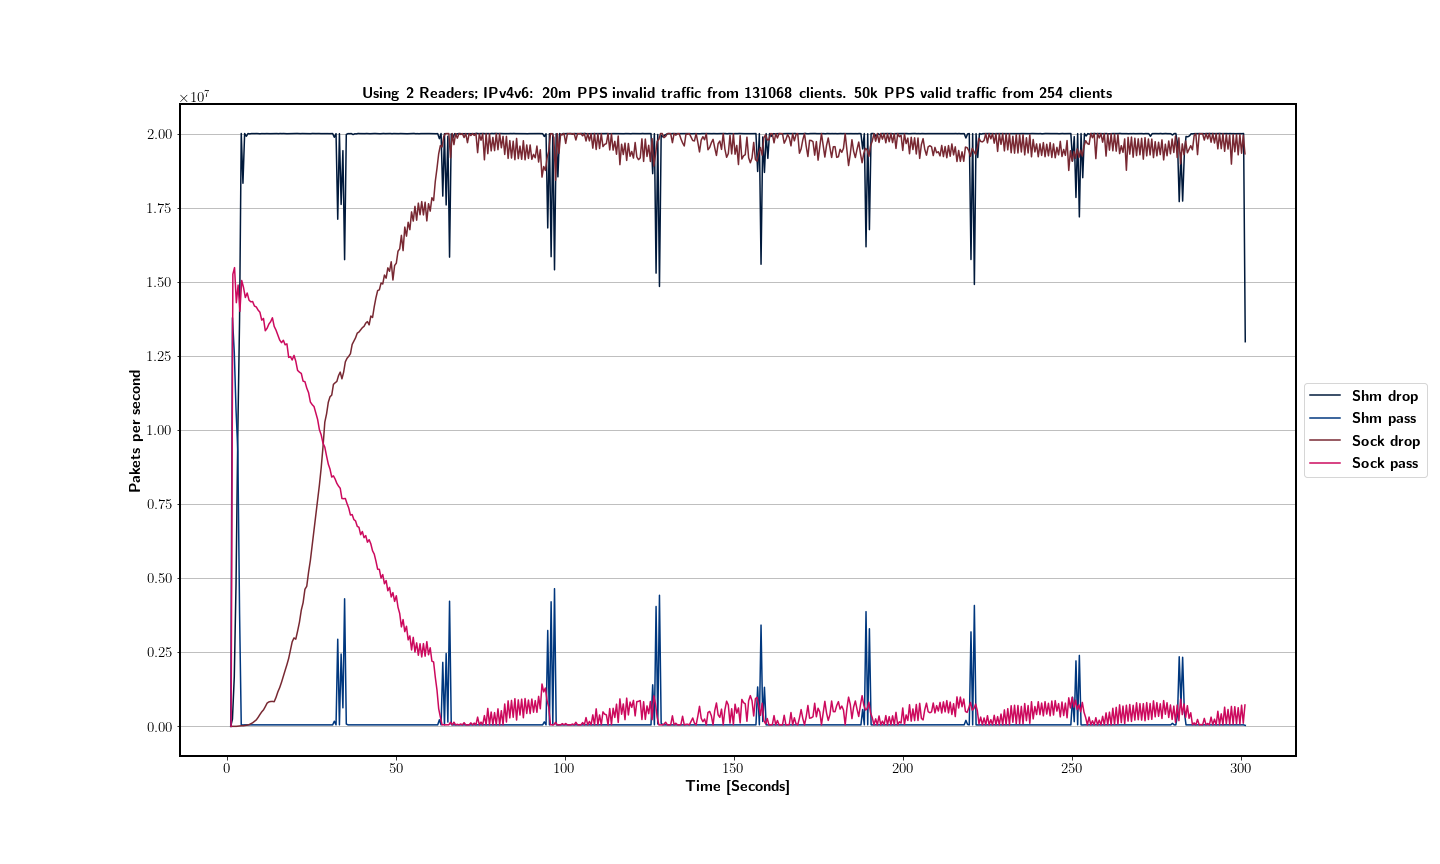
\includegraphics[width=1.2\textwidth]{images/IPv4v6_20m_2ndReader_1.png}}
	\end{tabular}
	\begin{tabular}{llll}
		\toprule
		\textbf{IPC type} & \textbf{XDP\_DROP [$10^8$]} & \textbf{XDP\_PASS [$10^6$]} & \textbf{Relative drop [\%]} \\ \midrule 
		Shm & 59,15 & 79,92 & 98,64873119 \\
        Sock & 52,45 & 624,81 & 87,47139407 \\
	\bottomrule
	\end{tabular}
    \begin{tabular}{llll}
		\toprule
		\textbf{IPC type} & \textbf{Packets received by udp\_server [$10^6$]} & \textbf{Log messages [$10^5$]} & \textbf{CPU [seconds]} \\ \midrule 
		Shm & 24,61 & 101,26 & 49.90 \\
        Sock & 11,32 & 65,01 & 251.49 \\
	\bottomrule
	\end{tabular}
	\caption[Simplefail2ban with 2nd Reader, IPv4v6, 20m \ac{PPS}, 131068 malicious clients]{Total packets sent: 6015m. Best-case drop rate: 99,934466\%}
	\label{fig:data:ipv4v6:20m:131068:2nd}
\end{figure}

That changes in figure \ref{fig:data:ipv4v6:30m:131068:2nd}.
Now, the socket \ac{IPC} type is unable to defend against the \ac{DoS} attack, and the system is overwhelmed - failing to drop all invalid traffic.  
The \texttt{relative drop} falls to approximately 54 percent, the number of messages passed to the kernel rise significantly and the application udp\_server is not able to handle the influx of incoming data.
Fewer log messages are sent to all readers and the \ac{CPU} time falls, likely due to the system not having any resources left for user space applications.
Meanwhile, the shared memory \ac{IPC} type performs just as well as in figure \ref{fig:data:ipv4v6:30m:131068}, when no second reader was attached to the \ac{IPC} architecture.

A difference of this scale was not initially expected.
However, increased performance of the shared memory \ac{IPC} type was attributed to the overwrite feature.
Enabling this feature meant that slower reader processes were ignored if they slowed down any writers.
The socket \ac{IPC} type cannot abandon slow readers, it has to wait for each reader to receive all data, unlike the shared memory \ac{IPC}.

\begin{figure}[!h]
	\centering
	\scriptsize
	\begin{tabular}{c}
    	\centerline{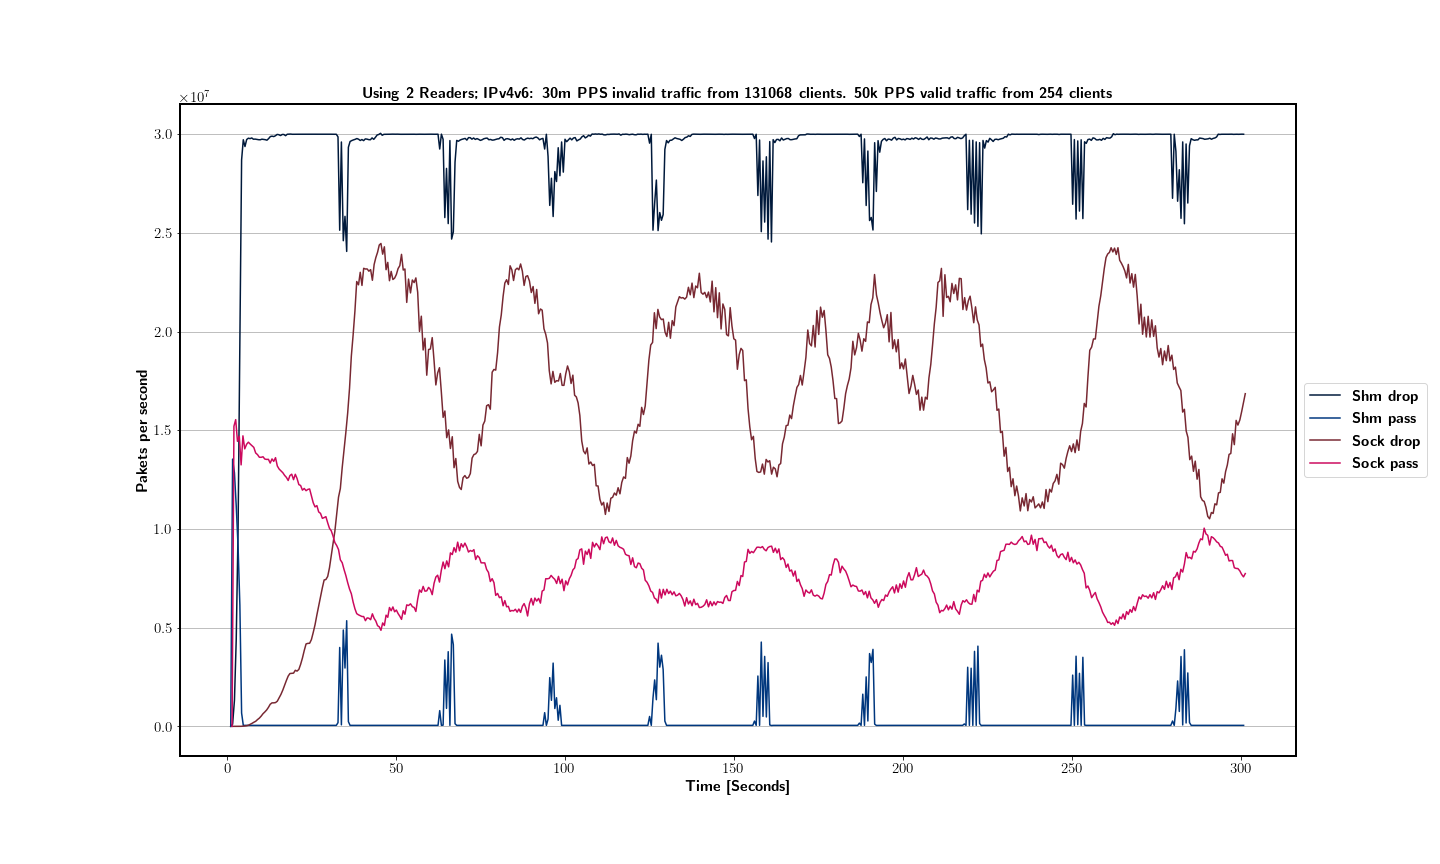
\includegraphics[width=1.2\textwidth]{images/IPv4v6_30m_2ndReader_1.png}}
	\end{tabular}
	\begin{tabular}{llll}
		\toprule
		\textbf{IPC type} & \textbf{XDP\_DROP [$10^8$]} & \textbf{XDP\_PASS [$10^6$]} & \textbf{Relative drop [\%]} \\ \midrule 
		Shm & 87,83 & 118,74 & 97,63360872 \\
        Sock & 48,80 & 2385,53 & 54,22323337 \\
	\bottomrule
	\end{tabular}
    \begin{tabular}{llll}
		\toprule
		\textbf{IPC type} & \textbf{Packets received by udp\_server [$10^6$]} & \textbf{Log messages [$10^5$]} & \textbf{CPU [seconds]} \\ \midrule 
		Shm & 24,70 & 108,17 & 94.60 \\
        Sock & 3,10 & 30,04 & 31.91 \\
	\bottomrule
	\end{tabular}
	\caption[Simplefail2ban with 2nd Reader, IPv4v6, 30m \ac{PPS}, 131068 malicious clients]{Total packets sent: 9015m. Best-case drop rate: 99,95631067\%}
	\label{fig:data:ipv4v6:30m:131068:2nd}
\end{figure}

Another experiment was conducted to confirm the link between enabling the overwrite feature and the increased performance of the shared memory \ac{IPC} type:
The shared memory \ac{IPC} type is used without having the overwrite feature enabled.
Expectations were, that having to wait for all reader processes to receive data would result in a performance decrease.
This measurement is displayed in figure \ref{fig:data:ipv4v6:30m:131068:2nd:NoOverwrite}.

No such decrease in performance was measured whatsoever.
The only logical conclusion is, that the shared memory \ac{IPC} type manages to supply multiple readers with faster data transfer than is required for even 30m incoming invalid \ac{PPS}.
The overwrite feature was not needed and had no real impact on performance.
Increased latency when using the socket \ac{IPC} type likely culminated to such a degree that supplying multiple readers with data was not feasible.

\begin{figure}[!h]
	\centering
	\scriptsize
	%\begin{tabular}{c}
    %	\centerline{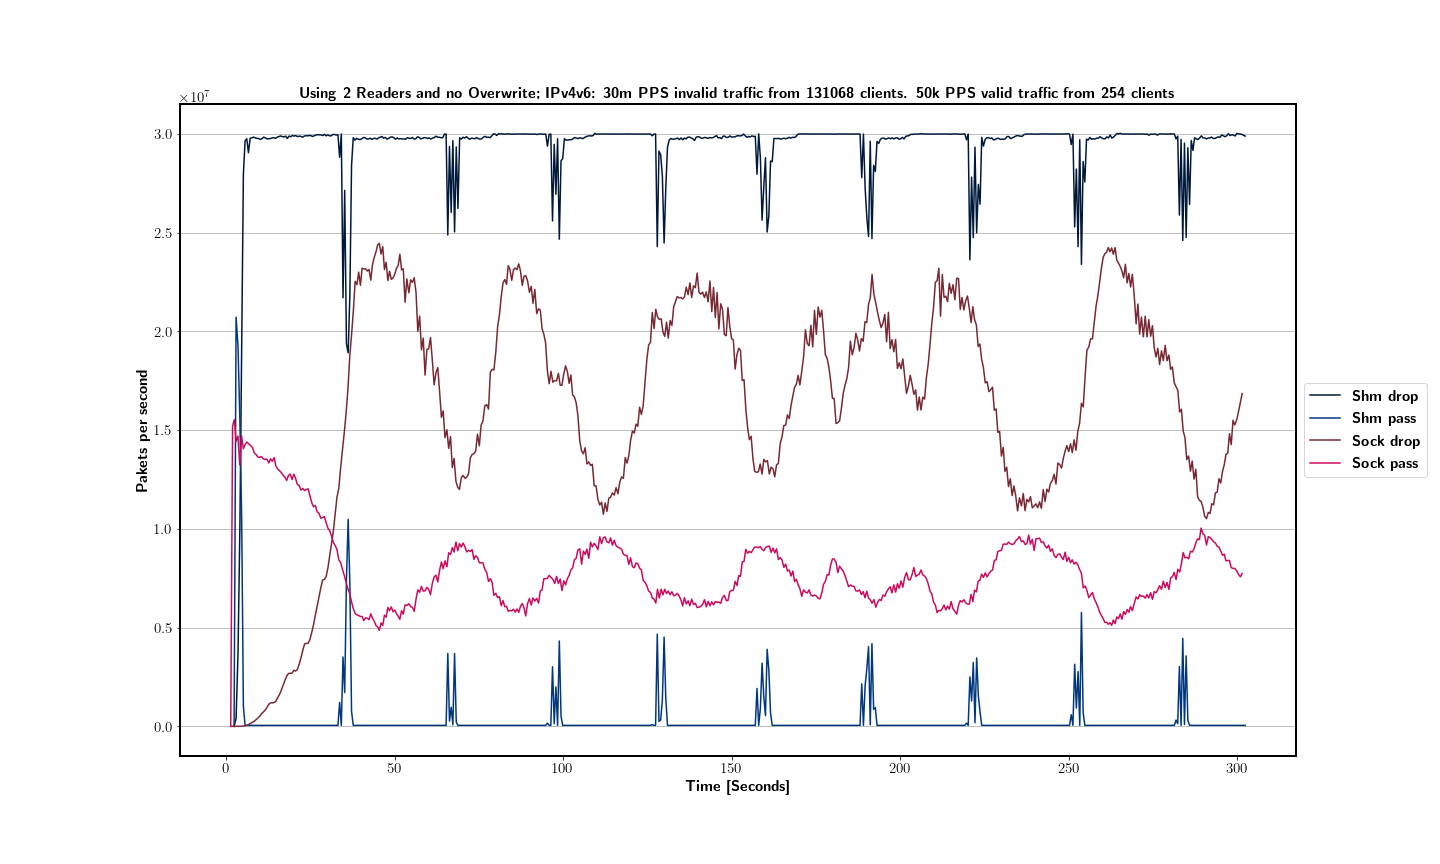
\includegraphics[width=1.2\textwidth]{images/IPv4v6_30m_2ndReaderNoOverwrite_1.png}}
	%\end{tabular}
	\begin{tabular}{llll}
		\toprule
		\textbf{IPC type} & \textbf{XDP\_DROP [$10^8$]} & \textbf{XDP\_PASS [$10^6$]} & \textbf{Relative drop [\%]} \\ \midrule 
		Shm & 87,99 & 125,56 & 97,81321365 \\
        Sock & 48,80 & 2385,53 & 54,22323337 \\
	\bottomrule
	\end{tabular}
    \begin{tabular}{llll}
		\toprule
		\textbf{IPC type} & \textbf{Packets received by udp\_server [$10^6$]} & \textbf{Log messages [$10^5$]} & \textbf{CPU [seconds]} \\ \midrule 
		Shm & 24,95 & 108,43 & 99.47 \\
        Sock & 3,10 & 30,04 & 31.91 \\
	\bottomrule
	\end{tabular}
	\caption[Simplefail2ban with 2nd Reader, IPv4v6, 30m \ac{PPS}, 131068 malicious clients]{Total packets sent: 9015m. Best-case drop rate: 99,95631067\%}
	\label{fig:data:ipv4v6:30m:131068:2nd:NoOverwrite}
\end{figure}